\newpage
\chapter{TINJAUAN PUSTAKA} \label{Bab II}

\section{Tinjauan Pustaka} \label{II.Tinjauan}
Berisi penelitian terdahulu yang menjadi konsep / pendukung penelitian yang dilakukan. Lakukan pembahasan secara sistematis dengan menjelaskan masalah apa yang diangkat di penelitian terdahulu, metode yang digunakan, kontribusi yang diberikan, serta analisis penulis terkait dengan keunggulan atau keterbatasannya. Tuangkan perbandingan penelitian terdahulu dengan penelitian yang akan dikerjakan, minimal 5 jurnal pembanding (4-5 tahun terakhir). Kemudian penulis sebaiknya melakukan rangkuman terutama terkait dengan peluang pengembangan atau tugas akhir yang akan dilakukan \par

Perujukan literatur dapat dilakukan dengan menambahkan entri baru dalam file \verb|references.bib|. Cara merujuk sitasi menggunakan \verb|\cite{nama label sitasi}|. Hasil sitasi seperti ini: \cite{knuth2001art}, \cite{Vogels2006Am}, atau \cite{Suryanto2019MAE}\cite{Ivanny2014Banding}. Daftar Pustaka hanya akan memunculkan sitasi yang direferensikan menggunakan command \verb|\cite{}|. \par

Tuliskan \textbf{judul jurnal, penulis jurnal, tahun jurnal terbit, penjelasan isi jurnal, metode penelitian, hasil penelitian \& pengujian}. \par
\begin{enumerate}[noitemsep]
	\item Sistem Informasi Pendaftaran Haji dan Umroh Di PT Multazam Sriwijaya Barakah Palembang Menggunakan Metode Rapid Application Development. \blindtext
	\item Sistem Informasi Umroh Di PT XYZ Lampung Menggunakan Metode Rapid Application Development. \blindtext
\end{enumerate}

Tabel ringkasan tinjauan pustaka ditulis setelah penjelasan masing-masing jurnal. \par
\begin{longtable}{| b{0.05\textwidth}|p{0.2\textwidth}|p{0.2\textwidth}|p{0.15\textwidth}|p{0.25\textwidth}|} % Longtable berguna agar tabel dapat terpotong di halaman baru
	\caption{Literasi Penelitian Terdahulu}
	\label{table:2.literasi}\\
	\hline
	\textbf{No.} & \textbf{Judul} & \textbf{Masalah} & \textbf{Metode} & \textbf{Hasil} \\
	\hline
	\endhead % Agar semua baris diatas ini diulang jika melewati halaman baru (repeat header row)
	1. & Sistem Informasi Pendaftaran Haji dan Umroh Di PT Multazam Sriwijaya Barakah Palembang Menggunakan Metode Rapid Application Development & Belum adanya sistem untuk pendaftaran haji \& umrah & Rapid Application Development & Sistem Informasi Pendaftaran Haji dan Umroh di PT Multazam Sriwijaya Barakah Palembang\\ 
	\hline
	2. & Sistem Informasi Umroh Di PT XYZ Lampung Menggunakan Metode Rapid Application Development & Belum adanya sistem untuk pendaftaran haji \& umrah & Rapid Application Development & Sistem Informasi Pendaftaran Umroh di PT XYZ Lampung\\ 
	\hline
	3. & Sistem Informasi Umroh Di PT XYZ Lampung Menggunakan Metode Rapid Application Development & Belum adanya sistem untuk pendaftaran haji \& umrah & Rapid Application Development & Sistem Informasi Pendaftaran Umroh di PT XYZ Lampung\\ 
	\hline
\end{longtable}

\section{Dasar Teori} \label{II.Teori}
Berisi teori/konsep yang berkaitan/digunakan dalam tugas akhir yang dikerjakan. Gunakanlah data melalui buku/jurnal referensi, publikasi tugas akhir, penelitian, buku, dan informasi web yang dapat dipertanggungjawabkan, hindari penggunaan dasar teori melalui tautan Wikipedia, surat kabar, atau portal berita, yang dapat memiliki isi yang tidak bersifat fakta. \par

\subsection{Teori 1} \label{II.Teori1}
Berikut adalah contoh penyisipan tabel menggunakan \verb|\begin{longtable}{}|: \par
	
	\begin{longtable}{|c|c|c|c|}
		\caption{Contoh Tabel}
		\label{table:2.contoh}\\
		\hline
		Col1 & Col2 & Col2 & Col3 \\
		\hline
		\endhead
		1 & 6 & 87837 & 787 \\ 
		\hline
		2 & 7 & 78 & 5415 \\
		\hline
		3 & 545 & 778 & 7507 \\
		\hline
		4 & 545 & 18744 & 7560 \\
		\hline
		5 & 88 & 788 & 6344 \\
		\hline
	\end{longtable}

\subsubsection{Subsubbab} \label{II.Teori1.1}
Berikut adalah contoh subsubbab. Ini adalah level subbab maksimal dalam laporan Tugas Akhir, dan tidak boleh lebih dalam. \par

Gambar \ref{fig:2.contoh} adalah contoh Gambar yang diambil dari internet yang harus dicantumkan sumbernya dan memiliki lisensi Creative Common. Jika gambar adalah milik peneliti lain atau tidak dibuat atau diambil sendiri maka peneliti wajib meminta izin kepada peneliti lain tersebut untuk mencantumkan gambar. Gunakan \verb|\begin{figure}| untuk memasukkan gambar. Gunakan \verb|\caption{[nama caption]}| untuk memberikan caption gambar. Nomor caption akan diurutkan secara otomatis. Jangan lupa untuk melabeli setiap gambar dengan \verb|\label{[nama label]}|, agar bisa direferensi menggunakan \verb|\ref{[nama label]}| \par
\begin{figure}[H] % Kalau menggunakan H, posisi gambar akan tepat dibawah teks
	\centering
	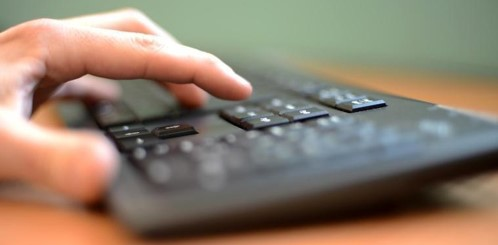
\includegraphics[width=0.6\textwidth]{figure/keyboard.jpg}
	\caption{Contoh gambar dan caption}
	\label{fig:2.contoh}
	{\footnotesize Sumber: Contoh} % Untuk memberikan sumber
\end{figure}

\subsection{Teori 2} \label{II.teori2}
Untuk membuat sebuah rumus persamaan, gunakan kode \verb|\begin{equationcaptioned}| seperti dibawah: \par
	
\begin{equationcaptioned}[eq:2.sederhana]{
	x + 1 = 2
}{
	Rumus sederhana % Caption rumus
}
\end{equationcaptioned}

Teks caption rumus tidak akan muncul di teks, tetapi akan muncul di Daftar Rumus. \par

\begin{equationcaptioned}[eq:2.mae]{
    MAE = \frac{1}{n} \sum_{i=1}^{n} \left| y_i - \hat{y}_i \right|
}{
    Mean Absolute Error (MAE)
}
\end{equationcaptioned}

Berikut adalah contoh penulisan persamaan yang lebih kompleks, yaitu persamaan distribusi normal. \par

\begin{equationcaptioned}[eq:2.mae]{
		P(x) = \frac{1}{{\sigma \sqrt {2\pi } }}e^{{{ - \left( {x - \mu } \right)^2 } \mathord{\left/ {\vphantom {{ - \left( {x - \mu } \right)^2 } {2\sigma ^2 }}} \right. \kern-\nulldelimiterspace} {2\sigma ^2 }}}
	}{
		Distribusi Normal
	}
\end{equationcaptioned}

Jika menuliskan banyak persamaan secara berurutan, gunakan  \verb|\begin{split}|: \par

\begin{equationcaptioned}[eq:2.mae]{
		\begin{split} 
			2x - 5y &=  8 \\ 
			3x + 9y &=  -12
		\end{split}
	}{
		Sistem persamaan linier
	}
\end{equationcaptioned}